\subsection{A Continuous Sequence and a Delayed Decision}
A fixed development trajectory illustrates the timing criterion
(Fig.~\ref{fig:reader-story}). The network continues moving after OFF;
a later event must be evaluated against that predicted response.
Under the tested out-of-bank network error, the bus-31 source is recovered
only after restoration. It is correct eventually and fails timely
attribution. The full development counts, active-mass trace, $\Delta M$
decomposition and failed admission control remain in the supplement.

\begin{figure*}[t]\centering
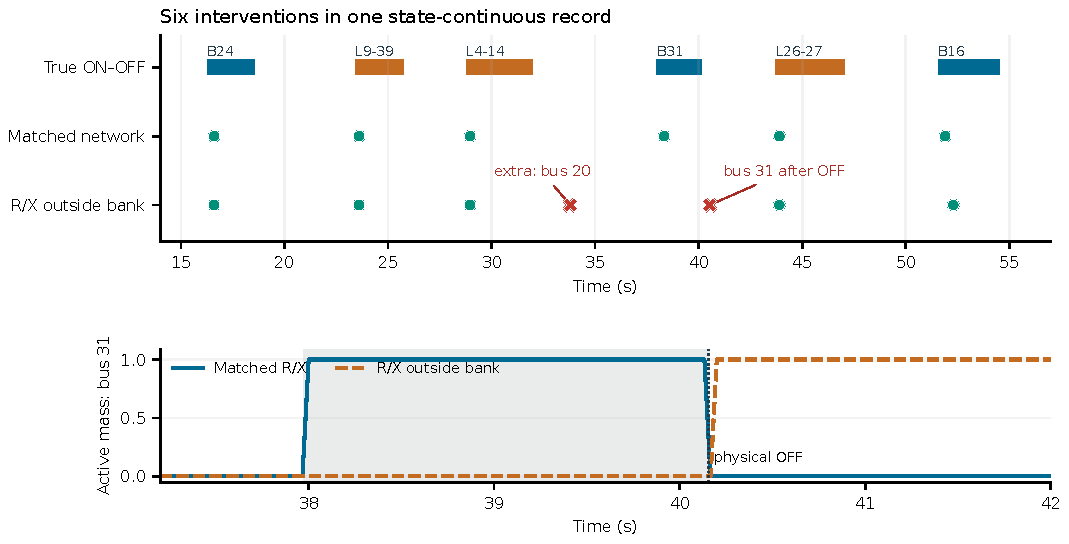
\includegraphics[width=.94\textwidth]{figures/generated/reader_episode_story.pdf}
\caption{One continuous development trajectory, shown for interpretation
rather than selected as an independent test. Top: physical ON--OFF
intervals and emitted diagnoses under matched and out-of-bank R/X.
Bottom: bus-31 active mass, with the true intervention shaded. A diagnosis
after OFF misses the timely endpoint even when it identifies the source.
True timing enters only this retrospective display.}
\label{fig:reader-story}\end{figure*}

\subsection{A Continuous Single-State Physical Control}
An existing open-development control retains one committed augmented
physical state through restoration, rather than resetting to equilibrium.
It uses the same nominal conditional plant and measurement operators,
profiles severity over short alternatives lasting at most 19 reports,
and applies the same six-report publication clock to all three procedures.
The short GLR achieves \SSSimpleTimely/\SSSimpleTotal{} timely decisions
with \SSSimpleExtras{} extras, versus \SSNomTimely/\SSNomTotal{} and
\SSNomExtras{} for the nominal history bank, and
\SSMixTimely/\SSMixTotal{} and \SSMixExtras{} for the five-model bank.
These 54 replays share three development parents; they are separate from
the independent test. Different evidence scores, search and severity
updates remain, so this is a preliminary continuous-observer comparison,
not an isolated causal effect of history retention. Its complete
equations and closure outcomes are in the supplement.
